\documentclass[pdf]{beamer}

\usetheme{Median}

\usepackage{graphicx}
\usepackage{pgfpages}
\usepackage{caption}
\usepackage{amsmath}
\usepackage{mathrsfs}
\usepackage{tensor}
\usepackage{tikz}
\usepackage{pgfplots}
\setbeameroption{show notes}


\newcommand{\credit}[1]{\tiny{\textcolor{blue}{Credit: #1}}}




\title[Stochastic signal originating from CGBs mesured by LISA]{Characterization of the stochastic signal originating from compact binary
populations as measured by LISA}
\subtitle{Nikolaos Karnesis, Stanislav Babak, Mauro Pieroni et al}
\author{MohammadReza Torkamani}

\begin{document}
\setbeamertemplate{caption}{\raggedright\insertcaption\par}

\begin{frame}
    \titlepage
\end{frame}

\begin{frame}{Table of Contents}
\vspace*{.1cm}
  \tableofcontents
\end{frame}
\section{Introduction}
\subsection{Gravitational waves}
\begin{frame}{Gravitational waves}
 \begin{columns}
 	\hspace{.5cm}
    \column[c]{0.5\textwidth}
    Ripples in space-time caused by accelerated masses.
        
	
	\begin{block}{Einstein field equations}
	\begin{equation*}
    \tensor{G}{_\mu_\nu} = \dfrac{8\pi G}{c^4} \tensor{T}{_\mu_\nu}  
    \end{equation*}
	\end{block}
	\begin{tiny}
	$G_{\mu\nu}$: Einstein tensor $\quad$ $T_{\mu\nu}$: Energy-Momentum tensor\\
	$G$: Gravitational constat $\quad$ $c$: speed of light
	\end{tiny}
	
	
    \begin{equation*}
    \tensor{g}{_\mu_\nu} = \tensor{\eta}{_\mu_\nu} + \tensor{h}{_\mu_\nu} \qquad |h|<<1 
    \end{equation*}
    \begin{equation*}
    \tensor{\bar{h}}{_\mu_\nu} = \tensor{h}{_\mu_\nu} -\dfrac{1}{2} \tensor{\eta}{_\mu_\nu} h  
    \end{equation*}
    
    
    \column{0.5\textwidth}
    \begin{figure}
    \includegraphics[scale=.14]{fig/GravWave.jpg}
    \caption*{\credit{R. Hurt (Caltech-IPAC)}}
    \end{figure}
  \end{columns}

\end{frame}

\begin{frame}{Gravitational waves}

	\begin{columns}
	\hspace{.5cm}
	\column[c]{0.5\textwidth}
	Lorenz gauge: $\partial_\mu \tensor{\bar{h}}{^\nu^\mu} = 0$
	\begin{block}{Wave equation}
	\begin{equation*}
	\Box \tensor{\bar{h}}{_\mu_\nu} = 0
	\end{equation*}		
	\end{block}
	
	\begin{equation*}
	\tensor{\bar{h}}{_\mu_\nu} = \tensor{A}{_\mu_\nu} \exp{(ik_\alpha x^\alpha)}
	\end{equation*}
	
	Transverse traceless gauge: $\tensor{\bar{h}}{_\mu_\nu} U^\mu = 0$ and $\tensor{\bar{h}}{_\mu^\mu} = 0$
	
	\column[c]{0.5\textwidth}
	
	\begin{align*}
	16 \xrightarrow{symetry} 10 \xrightarrow[gauge]{Lorenz} 6 \xrightarrow[gauge]{TT} 2
	\end{align*}		
	\begin{equation*}
	\tensor{h}{_\mu_\nu} = \begin{bmatrix}
	0&0&0&0\\
	0&h_+&h_\times&0\\
	0&h_\times&-h_+&0\\
	0&0&0&0
	\end{bmatrix}
	\end{equation*}		
	
\begin{figure}
 \scalebox{.5}{
\begin{tikzpicture}
  \begin{axis}[
    % Comment out or remove the following lines to hide the axes
    hide axis,
    ticks=none,
  ]

  % Plane 1
  \addplot3[fill=blue, opacity=.5, mesh, domain=-5:5, y domain=-5:5]
    {0};

  % Plane 2
  \addplot3[fill=red, opacity=.5, mesh, domain=-5:5, y domain=-5:5]
    {1};

  % Plane 3
  \addplot3[fill=green, opacity=.5, mesh, domain=-5:5, y domain=-5:5]
    {2};


	\draw[->, thick] (300,300,0) -- (300,300,260) node[above, right] {$U^\mu$};
  \end{axis}
  
\end{tikzpicture}}
\end{figure}		
	
	\end{columns}

\end{frame}

\subsection{Ground-based observatories}
\begin{frame}{LIGO Structure}
Giant Michelson interferometer
\begin{columns}
\column[c]{0.5\textwidth}
\begin{figure}
\includegraphics[scale=.6]{fig/HiResHanford_5.jpg}
\caption*{\credit{Caltech/MIT/LIGO Lab}}
\end{figure}
\column[c]{0.5\textwidth}
\begin{figure}
\includegraphics[scale=.14]{fig/IFO_SCHEME.png}
\caption*{\credit{D. V. Martynov et all, 2018}}
\end{figure}
\end{columns}
\begin{equation*}
S(t) = h(t) + n(t)
\end{equation*}
\end{frame}

\begin{frame}{LIGO Noise budget}
\begin{columns}
\column[c]{.65\textwidth}
\begin{figure}
\caption*{Hanford detector}
\includegraphics[scale=.17]{fig/noise-budget-ligo.png}
\caption*{\credit{Craig Cahillane et all, 2022}}
\end{figure}
\column[c]{.35\textwidth}

Dominant noise:

\begin{itemize}
\item  
Quantum shot in high frequency

\item  
seismic noise in low frequency
\end{itemize}

\end{columns}
\end{frame}

\begin{frame}{First detection (GW150914)}
\begin{figure}
\includegraphics[scale=.2]{fig/GW150914.png}
\caption*{\credit{B. P. Abbott et al., 2016}}
\end{figure}
\end{frame}

\subsection{LISA}
\begin{frame}{Laiser Interferometer Space Antenna (LISA)}
\begin{columns}

\column[c]{0.5\textwidth}
\begin{figure}
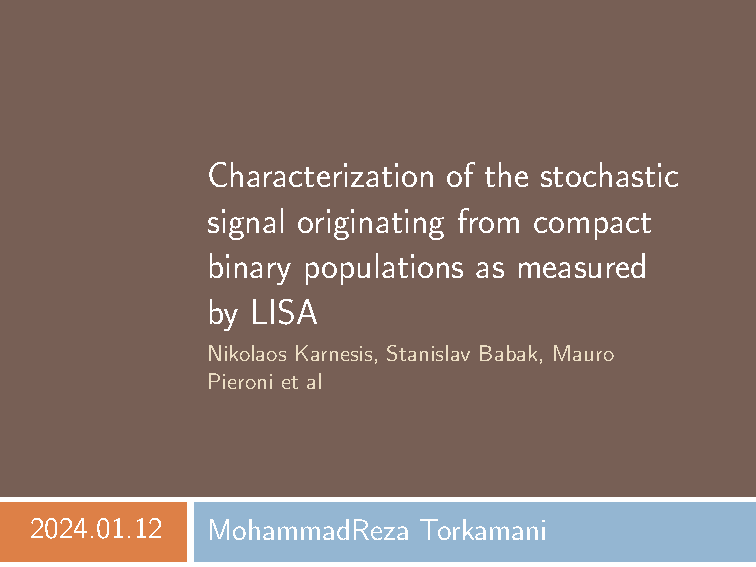
\includegraphics[scale=.15]{fig/LISA.png}
\caption*{\credit{Karsten Danzmann et al., 2017}}
\end{figure}

\column[c]{0.5\textwidth}
\begin{figure}
\includegraphics[scale=.12]{fig/LISAsch.png}
\caption*{\credit{Jean-Baptiste Bayle et al., 2021}}
\end{figure}

\end{columns}
\end{frame}

\begin{frame}{LISA Band}
\begin{figure}
\includegraphics[scale=.2]{fig/observedLISA.png}
\caption*{\credit{Karsten Danzmann et al., 2017}}
\end{figure}
\end{frame}

\begin{frame}{LISA Band}
GW sources in LISA band
\begin{itemize}
\item Supermassive black hole binaries (SMBHBs)
\item Stellar-mass black hole binaries (SBBHs)
\item Ultracompact galactic binaries (CGBs)
\item Verification galactic binaries
\item extreme mass ratio inspiral (EMRIs)
\item stochastic GW background 
\end{itemize}
\end{frame}

\begin{frame}{LISA Isuues}
\begin{itemize}
\item LISA data are expeted to be signal dominated
\item LISA sources are expected to be long-lived
\item GW signals will be overlapping in time(frequency)
\pause
\item Some signals can be resolvable due to high signal to noise ratio
\pause
\item remaining signals will affect the sensitivity as extra noise (confusion noise)
\end{itemize}
\end{frame}

%%%%%%%%%%%%%%%%%%%%%%%%%%
%%%%%%%%%%%%%%%%%%%%%%%%%%
\section{Methodology}
\begin{frame}{Overview}
\begin{itemize}
\item Simulating around 30 milion CGBs from Radler LISA data challenge dataset
\item Simulating the instumental noise using the LISA code simulatior
\item For each $T_{obs}$ gererate the idealized dataset in the frequency domain
\item Apply the method to find the final sensitivity
\item Fit the data with theoretical curve
\end{itemize}
\end{frame}

\begin{frame}{Methode}
\begin{itemize}
\item Assumpion: Bright sources with a signal-to-noise ratio larger than a given threshold are detected and charachterized without systematic bias or source cofusion.
\end{itemize}
\begin{block}{SNR}
\begin{align*}
\rho^2_{tot} &= \sum_k (h_k|h_k), \quad  \text{k:noise-orthogonal TDI variables} \\
h_k|h_k &= 4 \int_{0}^{\infty} df \dfrac{|\tilde{h}_k(f)|^2}{\tilde{S}_n(f)}, \quad \tilde{S}_n(f):\text{one-sided PSD} \\
\tilde{S}_n(f) &= \tilde{S}_{instr}(f) +\tilde{S}_{conf}(f)
\end{align*}
\end{block}
\end{frame}

\begin{frame}{Methode}
\begin{enumerate}
\item Simulating 30 milions CGBs
\item Calculating the PSD of the signal and the instrumental noise
\item Calculating the SNR of each source with respect to the instrumental noise ($\rho_i^{iso}$)
\item Stimating the SNR of each source using either a running mean or median on the power spectrum of the data ($\rho_i$)
\item If $\rho_i > \rho_0$ the source will be subtracted from the data
\item Iterate the process until no sources exceed the threshold ($\rho_0$)
\end{enumerate}
\end{frame}

\section{Result}
\subsection{CGBs}
\begin{frame}{Compact Galactic Binaries}
\begin{figure}
\includegraphics[scale=.22]{fig/MainPSD.png}
\caption*{\credit{Nikolaos Karnesis et al, 2021}}
\end{figure}
\end{frame}


\begin{frame}{Compact Galactic Binaries}
Analytical model for the estimated confusion foreground:
\begin{block}{Confusion foreground model}
\begin{equation*}
S_{gal}  = \dfrac{A}{2} f^{-7/3} e^{-(f/f_1)^\alpha} (1+\tanh((f_{knee}-f)/f_2))
\end{equation*}
\end{block}
$A$: Amplitude $\qquad$ $f_1, f_2$ and $f_{knee}$: Scaling frequencies \\
$f$: Frequency $\qquad$ $\alpha$: Smoothness parameter 

Approximation for $f_1$ and $f_{knee}$:
\begin{align*}
\log_{10}(f_1) = a_1 \log_{10}(T_{obs}) +b_1\\
\log_{10}(f_{knee}) = a_k \log_{10}(T_{obs}) + b_k 
\end{align*}
$a_1, b_1, a_k$ and $b_k$ are amplitude calibration parameters
\end{frame}

\begin{frame}{Compact Galactic Binaries}
\begin{columns}
\column[c]{.55\textwidth}
\begin{figure}
\includegraphics[width = \textwidth]{fig/FittingPSD.png}
\caption*{\credit{Nikolaos Karnesis et al, 2021}}
\end{figure}
\column[c]{.45\textwidth}
\begin{figure}
\includegraphics[width = \textwidth]{fig/Table2.png}
\end{figure}
\begin{figure}
\includegraphics[width = \textwidth]{fig/Table1.png}
\end{figure}

\end{columns}
\end{frame}

\subsection{SBBHs}
\begin{frame}{Stellar-mass binaries black hole}
\begin{itemize}
\item LISA is sensitive to the early inspiral stage of orbit evolution of SBBHs
\item They appear in the high-frequency tail of LISA band until ($3\mathrm{mHz}$)
\item There is a very low chance for the transition of SBBHs from LISA band to LIGO band during the LISA observation time
\item The population of SBBHs observed by LISA depends on the merger rate of SBBHs ($\mathcal{R}$)
\item $\mathcal{R}$ can be stimated from data of ground-base observatories
\end{itemize}
\end{frame}

\begin{frame}{Stellar-mass binaries black hole}
\begin{itemize}
\item Observation time of $T_{obs} \sim 2.7$ yr
\item Simulating the dataset using PhenomD waveform model (S. Khan et al, 2016)
\item Doing the same process as CGBs
\end{itemize}
\end{frame}

\begin{frame}{Stellar-mass binaries black hole}
\begin{figure}
\includegraphics[width=.8\textwidth]{fig/SMBHs.png}
\caption*{\credit{Nikolaos Karnesis et al, 2021}}
\end{figure}
\end{frame}


\subsection{Combining the populations}
\begin{frame}{Combining the populations}
\begin{itemize}
\item Doing the same process again!
\item Instead of iterating over one type, iterate over all types
\item Comparing SNR of each type with itself
\item Final result is just superposition of the foreground signals from all given types of sources
\begin{block}{Superposition}
\begin{equation*}
\tilde{S}_n(f) = \tilde{S}_{instr}(f) +\sum_t \tilde{S}_{conf,t}(f)
\end{equation*}
\end{block}
\end{itemize}
\end{frame}

\begin{frame}{Combining the populations}
\begin{figure}
\includegraphics[width=.9\textwidth]{fig/combin.png}
\caption*{\credit{Nikolaos Karnesis et al, 2021}}
\end{figure}
\end{frame}


\section{Conclusion}
\begin{frame}{Conclusion}
\begin{itemize}
\item SBBHs is not strong enough to affect the final result
\item Due to the presence of CGBs the most sensitive firequency of LISA is moved to the right
\end{itemize}
\end{frame}

\begin{frame}
\begin{center}
\Huge Thank you!
\end{center}
\end{frame}

\begin{frame}{PSD}
\begin{figure}
\includegraphics[scale=.2]{fig/PSD-TOT.png}
\caption*{\credit{C J Moore et al, 2014}}
\end{figure}
\end{frame}

\begin{frame}{Characteristic strain}
\begin{figure}
\includegraphics[scale=.2]{fig/Char-TOT.png}
\caption*{\credit{C J Moore et al, 2014}}
\end{figure}
\end{frame}

\begin{frame}{Dimensionless energy density}
\begin{figure}
\includegraphics[scale=.2]{fig/Energy-TOT.png}
\caption*{\credit{C J Moore et al, 2014}}
\end{figure}
\end{frame}

\begin{frame}{TDI}
\begin{columns}
\column[c]{.5\textwidth}
\begin{figure}
\includegraphics[scale=.15]{fig/LISAschem.png}
\caption*{\credit{Massimo Tinto et al, 2020}}
\end{figure}
\column[c]{.5\textwidth}
\begin{figure}
\includegraphics[scale=.15]{fig/Distance.png}
\caption*{\credit{Olaf Hartwig, 2021}}
\end{figure}
\end{columns}
\end{frame}

\end{document}
